\documentclass[10pt]{beamer}
\usepackage[utf8]{inputenc}
\usetheme{metropolis}
\usecolortheme{beaver}
\title{GEN-I: Nelinearne transakcije}
\author{\centering Anja Trobec \\ Mentor: David Grgič}
\vspace{3pt}
\institute{\centering Fakulteta za Matematiko in Fiziko}
\date{\centering Maj, 2022}

\begin{document}

\frame{\titlepage}

\begin{frame}
\frametitle{Navodila za izdelavo projekta}
\begin{itemize}
\item{Imamo mesečno nelinearno transakcijo za električno energijo, kjer se lahko znotraj določenih omejitev za vsako uro znotraj meseca dobave lastnik opcijskosti odloči, koliko el. energije bo prevzeli/dobavil. }
\item{Transakcijo ovrednotimo napram množici cenovnih scenarijev, tako da za vsak cenovni scenarij dobimo njen profit. Cenovni scenariji so možne prihodnje cene dobave.}
\item{Za to transakcijo želimo poiskati njen ekvivalent standardne Evropske opcije.}
\item{Kakšni so parametri ekvivalenta te opcije, kot količina, cena (strike), stran (nakup/prodaja) in tip (call/put) opcije?}
\end{itemize}
\end{frame}


\begin{frame}
\frametitle{Teoretični uvod}
\begin{itemize}
\item{Vhodni podatki so pari sestavljeni iz cene in profita pri dani ceni: $$(S_t,V_t).$$}
\item{Iščemo standardno Evropsko opcijo, ki najbolje aproksimira dane podatke.}
\item{Določiti je potrebno ali gre za \it{call} ali \it{put} opcijo.}
\item{Ali opcijo kupimo \it{angl. option buyer} ali opcijo prodamo \it{angl. option writer}. }
\item{Iskani parametri:
\begin{enumerate}
\item{izvršilno ceno (\it{angl. strike price}) $K$,}
\item{količino $Q$ in}
\item{opcijsko premijo (\it{angl. option premium}).} 
\end{enumerate}
}
\end{itemize}
\end{frame}


\begin{frame}
\frametitle{NAKUP EVROPSKE CALL OPCIJE}
\textbf{Call opcija} podeljuje \textbf{lastniku (kupcu opcije)} pravico
za nakup določenega inštrumenta (\emph{angl. underlying asset}) po
vnaprej določeni izvršilni ceni na določen dan. 

Lastniku call opcija ne predstavlja obveznosti, pač pa
priložnost (rečemo, da mu nudi opcijskost), da opcijo izvrši v primeru,
če cena inštrumenta na trgu naraste. Za call opcijo rečemo, da je:

\begin{itemize}
\item
  \textbf{in the money} - kadar je cena inštrumenta nad izvršilno ceno,
\item
  \textbf{at the money} - kadar sta cena inštrumenta in izvršilna cena
  enaki,
\item
  \textbf{put of the money} - kadar je cena instumenta pod izvršilno
  ceno.
\end{itemize}

Opazimo, da ima kupec evropske call opcije \textbf{neomejen dobiček} in
na drugi strani \textbf{izgubo omejeno s plačano premijo}.
\end{frame}


\begin{frame}
\frametitle{NAKUP EVROPSKE PUT OPCIJE}
\textbf{Put opcija} podeljuje \textbf{lastniku (kupcu opcije) } pravico
za prodajo določenega inštrumenta po vnaprej določeni izvršilni ceni na
določen dan. 

Lastniku call opcija ne predstavlja
obveznosti, pač pa priložnost, da opcijo
izvrši v primeru, če cena inštrumenta na trgu pade.

Za put opcijo rečemo, da je:

\begin{itemize}
\item
  \textbf{in the money} - kadar je cena inštrumenta pod izvršilno ceno,
\item
  \textbf{at the money} - kadar sta cena inštrumenta in izvršilna cena
  enaki,
\item
  \textbf{put of the money} - kadar je cena instumenta nad izvršilno
  ceno.
\end{itemize}

Kupec evropske put opcije ima \textbf{neomejen dobiček} in na drugi strani
\textbf{izgubo omejeno s plačano premijo}.
\end{frame}


\begin{frame}
\frametitle{PRODAJA EVROPSKE CALL OPCIJE}

Zdaj se postavimo v vlogo izdajatelja opcije. S tem ko \textbf{opcijo
prodamo}, zanjo \textbf{prejmemo premijo} in se zavežemo k izplačilu v
primeru, da kupec opcijo ob dospelosti izvrši. 

Torej je v primeru
prodaje call opcije \textbf{dobiček navzgor omejen s prejeto premijo} in
\textbf{izguba navzdol neomejena}.

\end{frame}

\begin{frame}
\frametitle{PRODAJA EVROPSKE PUT OPCIJE}

Zadnji scenarij pa je prodaja evropske put opcije. Kot izdajatelj put
opcije, \textbf{opcijo prodamo}, zanjo \textbf{prejmemo premijo} in se
zavežemo k izplačilu v primeru, da lastnik opcijo ob dospelosti izvrši.

Ponovno je \textbf{izguba navzdol neomejena}, medtem ko je
\textbf{dobiček navzgor omejen s prejeto premijo}.
\end{frame}


\begin{frame}
\frametitle{STANDARDNE EVROPSKE OPCIJE}
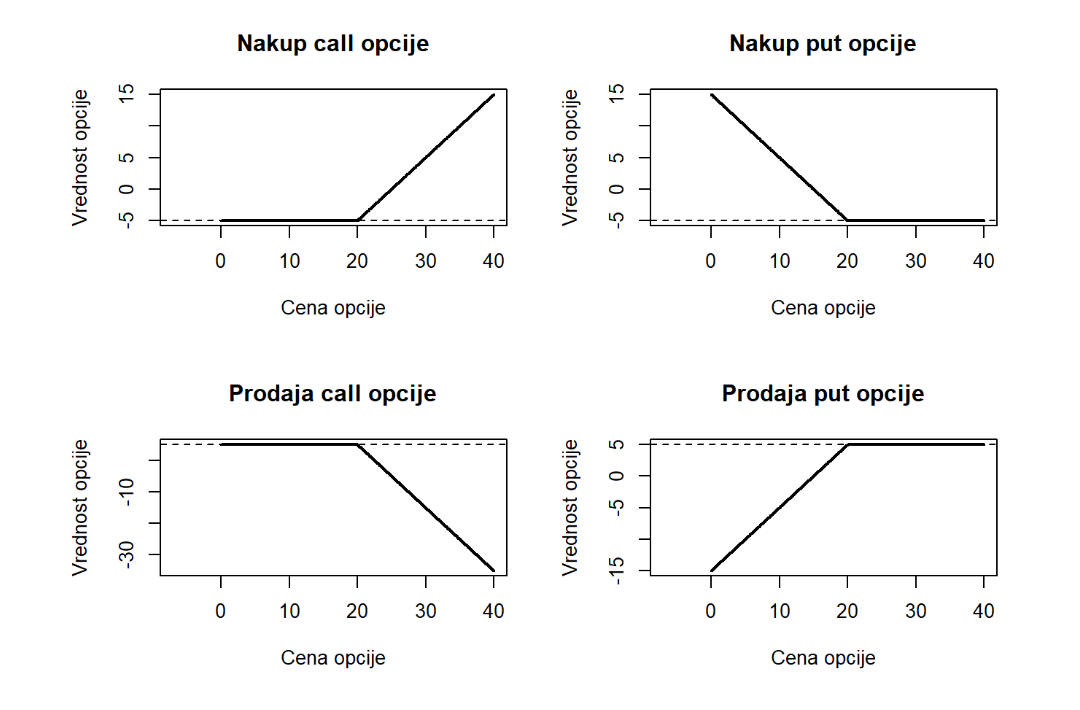
\includegraphics[width=1\textwidth]{vse4.png}
\end{frame}


\begin{frame}
\frametitle{PRISTOP K REŠEVANJU PROBLEMA}
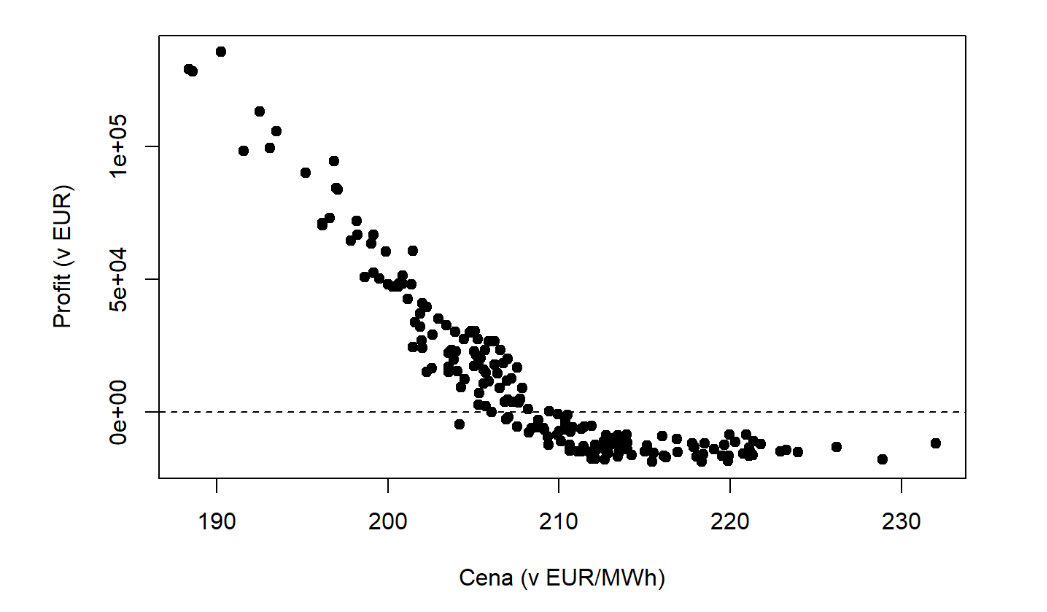
\includegraphics[width=1\textwidth]{zacetek.png}
\end{frame}


\begin{frame}
\frametitle{PRISTOP K REŠEVANJU PROBLEMA}
\begin{itemize}
\item{Ideja je, da \textbf{vsako vhodno transakcijo
aproksimiramo s kombinacijo dveh premic}. }

\item{Ugotovimo, za katero vrsto
opcije in tip pozicije gre.}

\item{Nadaljno lahko iz smernega koeficienta in
začetne vrednosti izbranih optimalnih premic, določimo iskane parametre.}
\end{itemize}
Premica, ki bo vselej vodoravna določa premijo: \[ y =  premija \]

Premica s pozitivnim ali negativnim naklonom določa količino (Q):

\[ y =  Q * S_t + n\]

Iz presečišča zgornjih dveh premic dobimo izvršilno ceno (K):

\[ K = \frac{premija - n}{Q} \]
\end{frame}


\begin{frame}
\frametitle{ALGORITEM}
\begin{itemize}
\item{Algoritem sprejme csv datoteko sestavljeno iz dveh stolpcev. \\
V prvem
stolpcu najdemo ceno inštrumenta izrazeno v EUR/MWh in v drugem stolpcu
najdemo izplačilo pri dani ceni, izrazeno v EUR. }
\item{Na prvem mestu nas zanima korelacija med podatki.}
\end{itemize}
\end{frame}


\begin{frame}
\frametitle{Pozitivna korelacija}
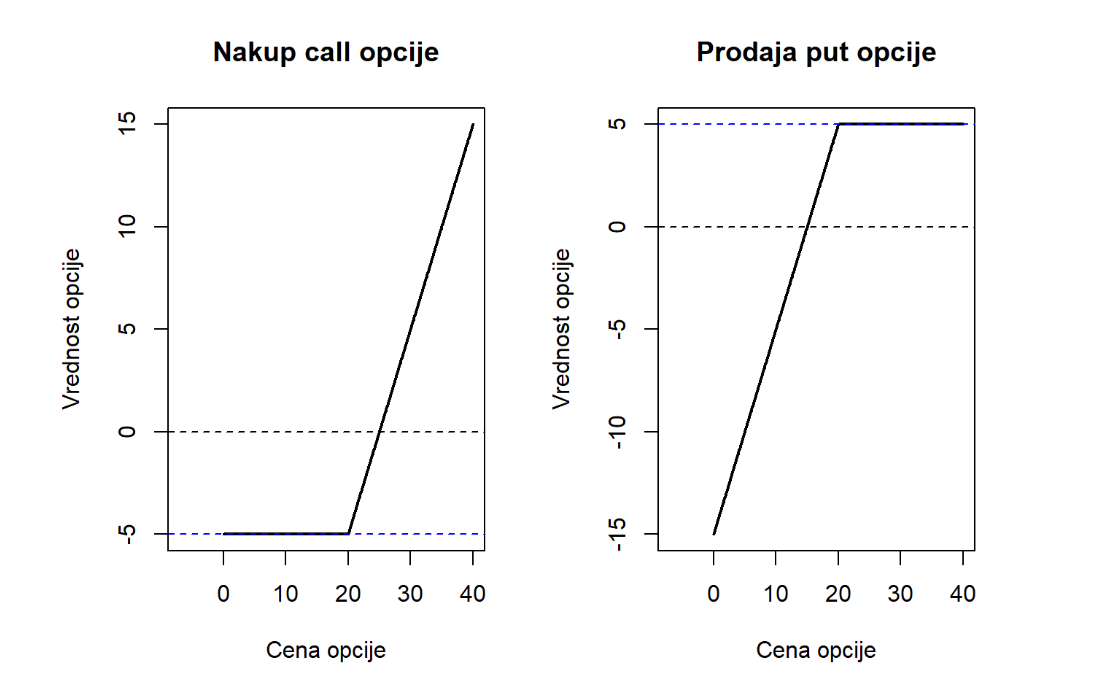
\includegraphics[width=1\textwidth]{neg_kor.png}

\end{frame}


\begin{frame}
\frametitle{Negativna korelacija}
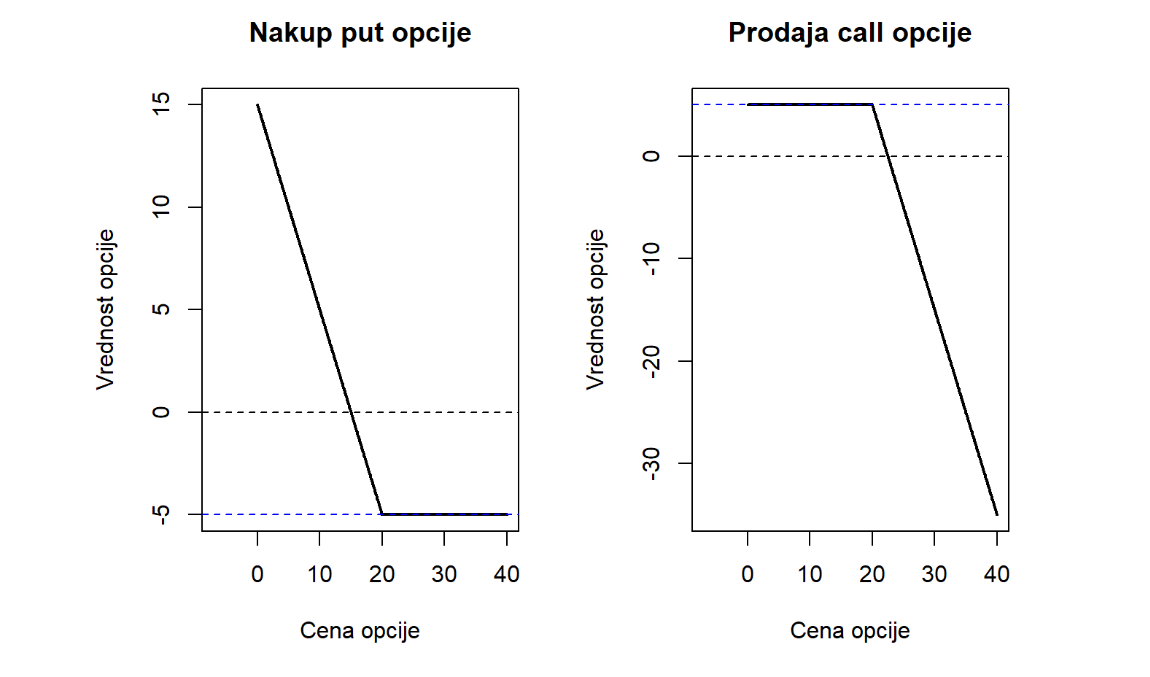
\includegraphics[width=1\textwidth]{poz_kor.png}
\end{frame}

\begin{frame}
\frametitle{ALGORITEM - optimalno prileganje}
\begin{itemize}
\item{\textbf{Iščemo optimalno prileganje izbrane opcije na dane podatke}. To storimo s pomočjo dveh premic.}
\item{Vodoravna premica - povprečje profitov.}
\item{Premica z neničelnim naklonom - linearna regresija.}
\item{Lastnosti premic in njuno presečišče.}
\end{itemize}
\end{frame}

\begin{frame}
\frametitle{PRIMER 1}
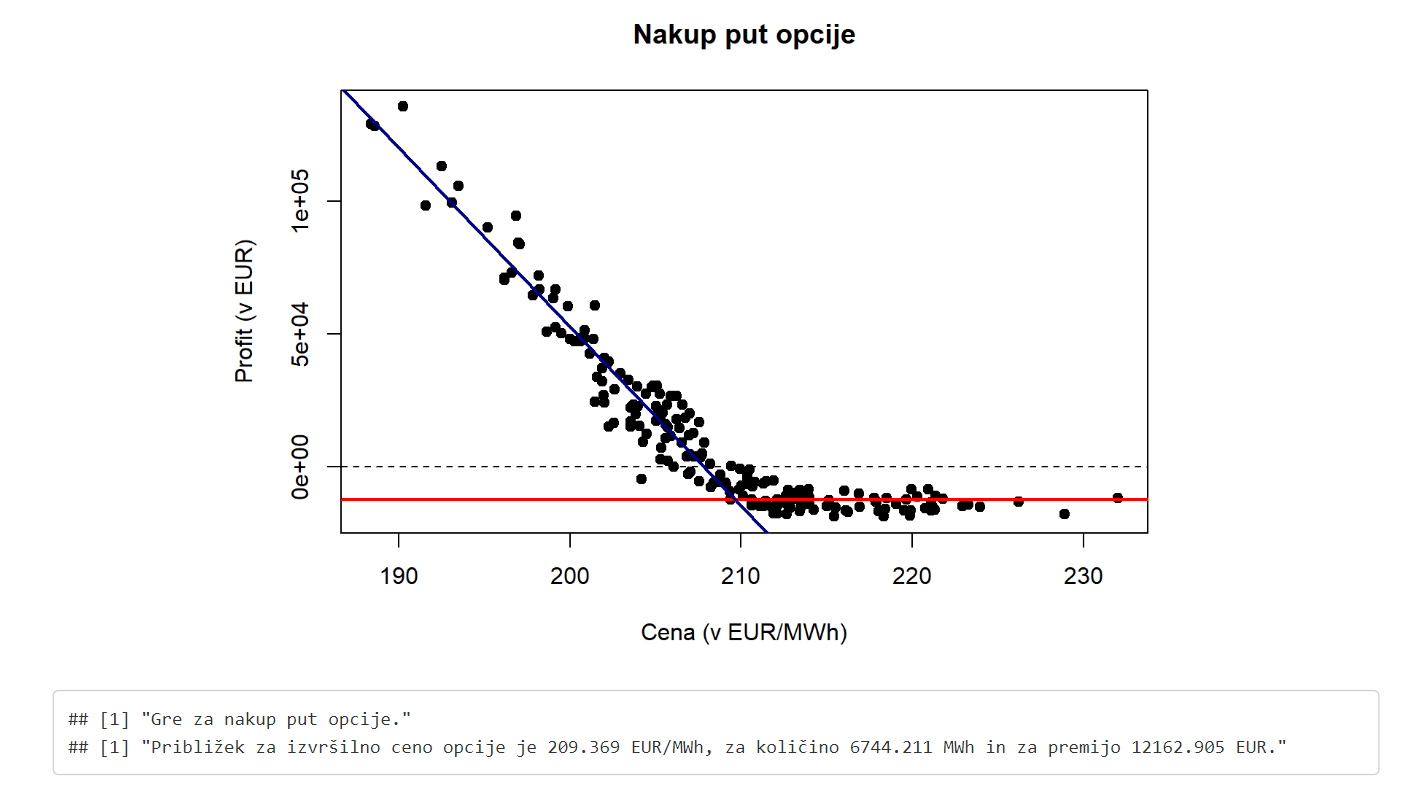
\includegraphics[width=1\textwidth]{primer1.png}
\end{frame}

\begin{frame}
\frametitle{PRIMER 2}
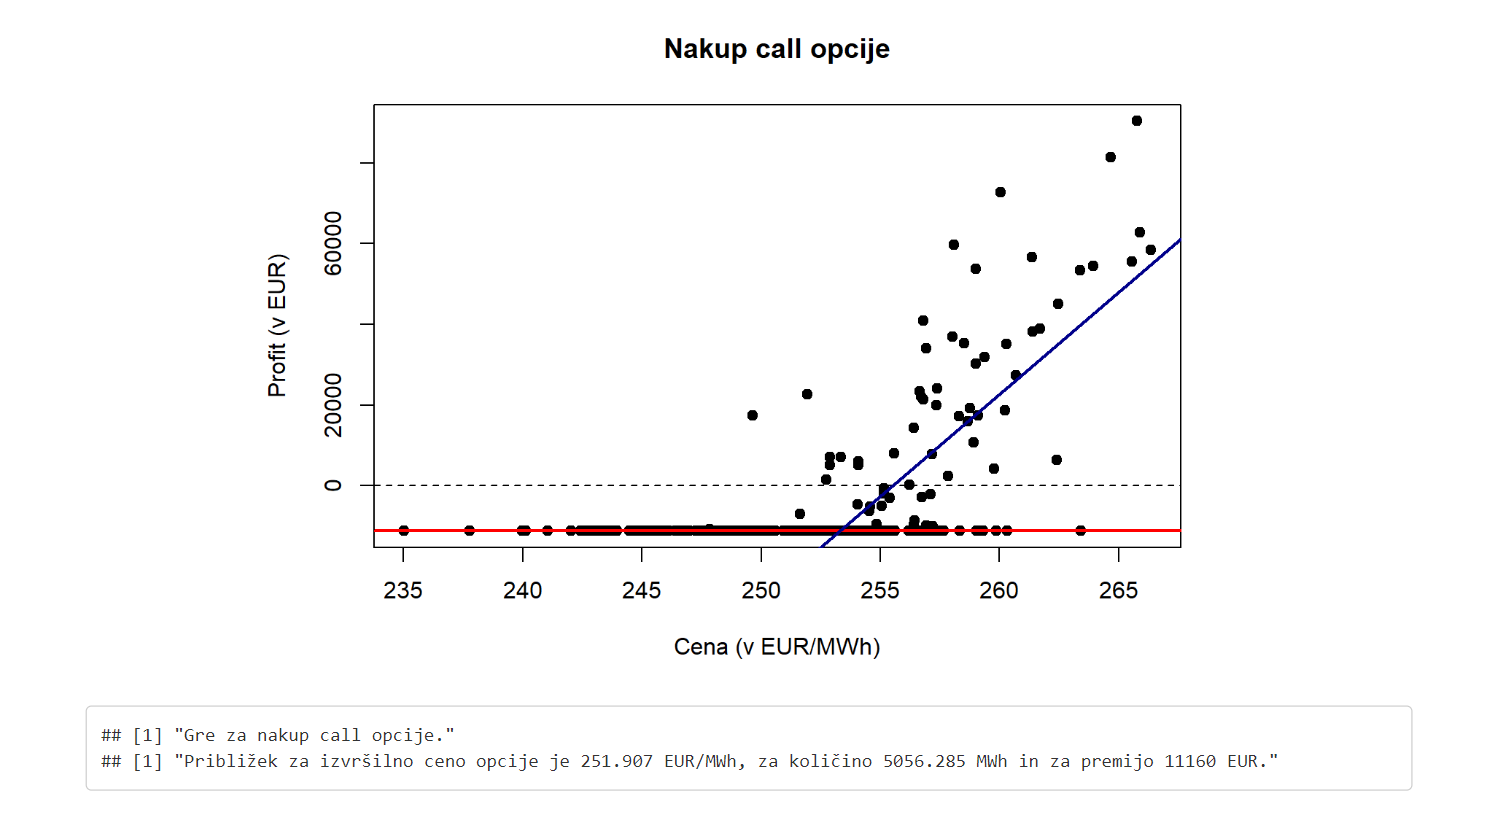
\includegraphics[width=1\textwidth]{primer2.png}
\end{frame}

\begin{frame}
\frametitle{PRIMER 3}
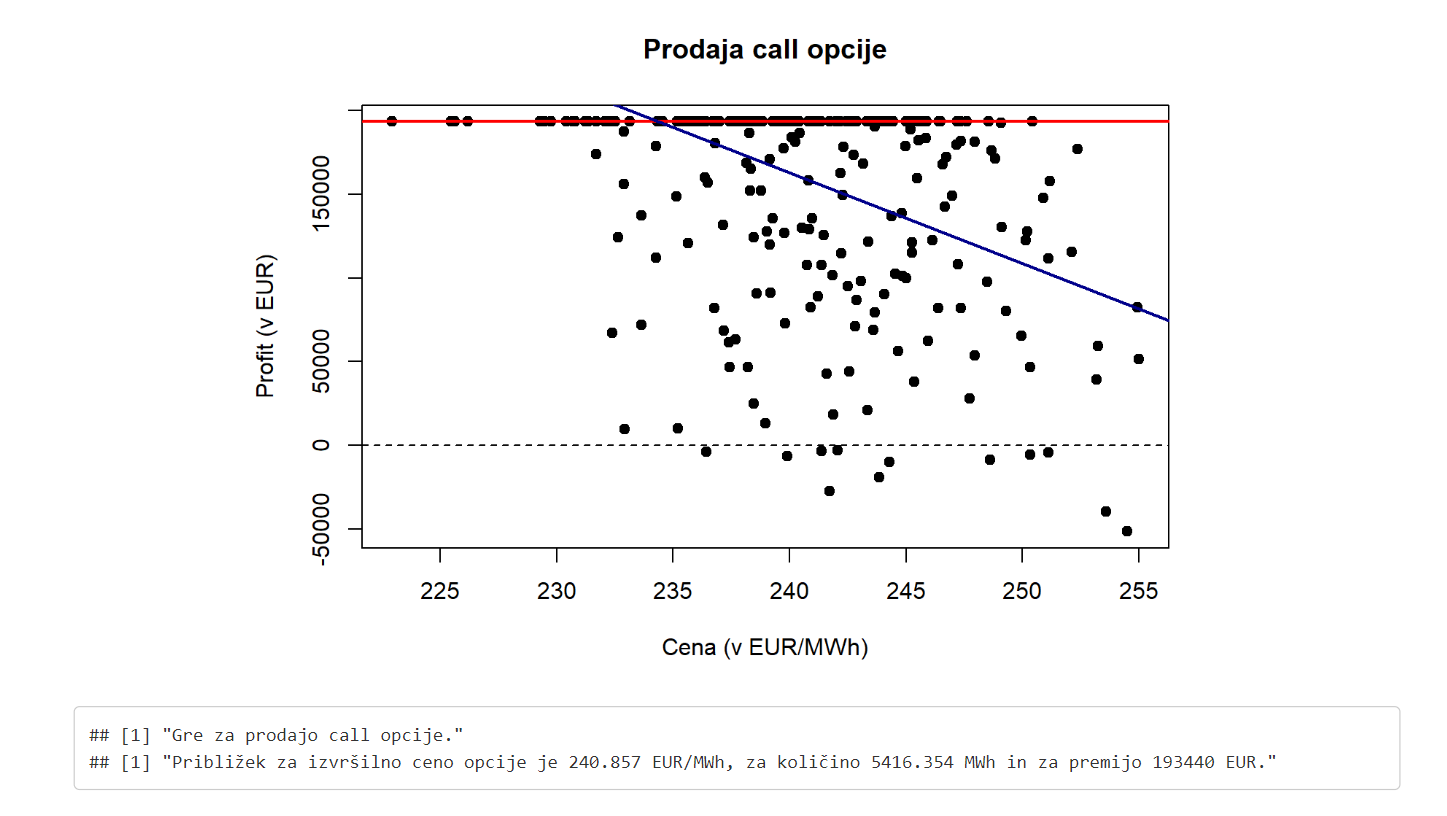
\includegraphics[width=1\textwidth]{primer3.png}
\end{frame}

\begin{frame}
\frametitle{PRIMER 4}
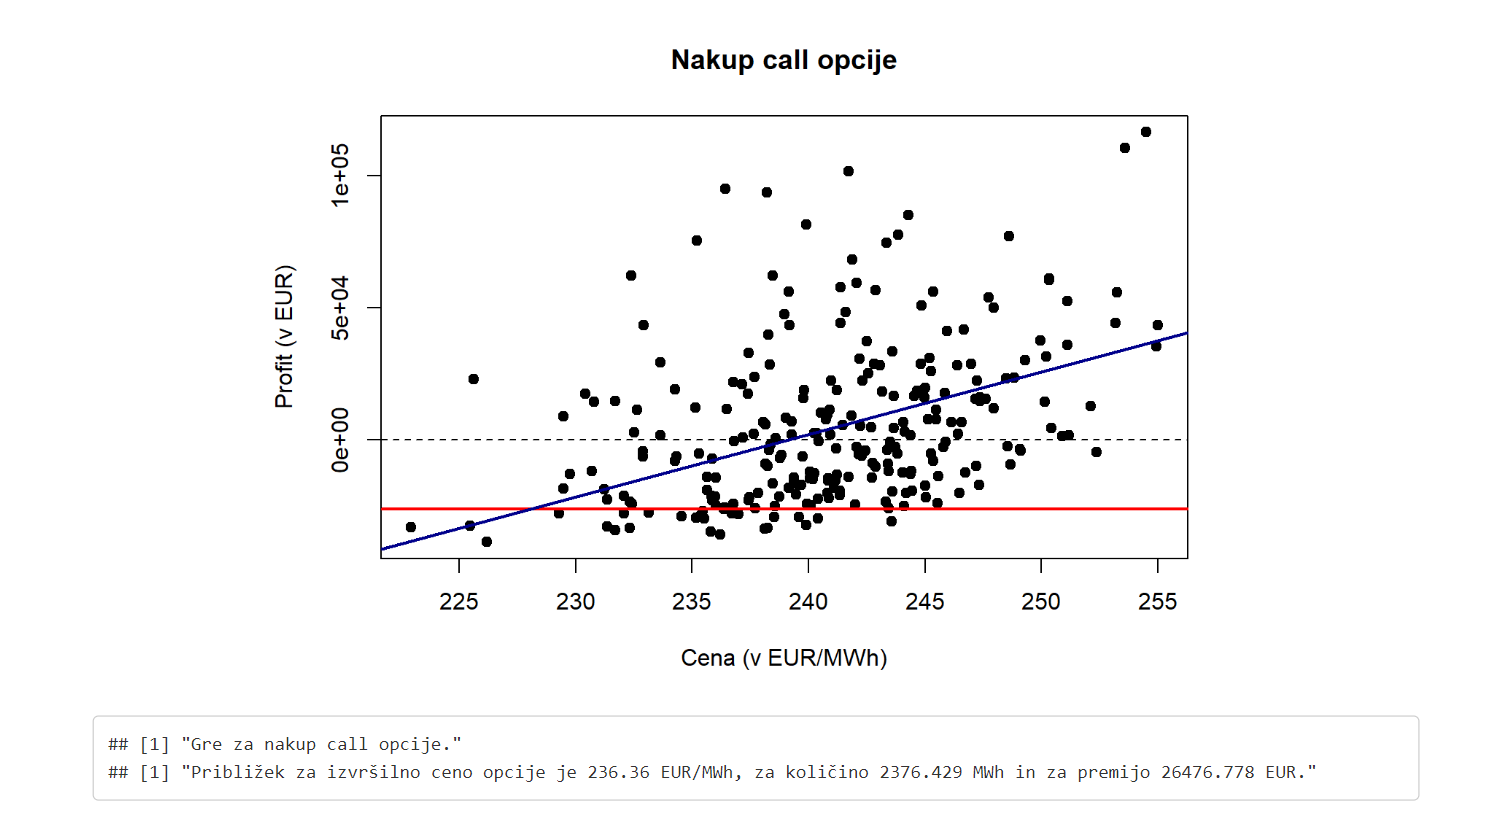
\includegraphics[width=1\textwidth]{primer4.png}
\end{frame}

\begin{frame}
\frametitle{Shiny aplikacija}

\end{frame}
\end{document}